\documentclass[main.tex]{subfiles}
%\usepackage{xr}
%\externaldocument{results}
\begin{document}
\chapter{Solution Plots}


\begin{figure}[h!]
\begin{subfigure}{1\textwidth}
\centering
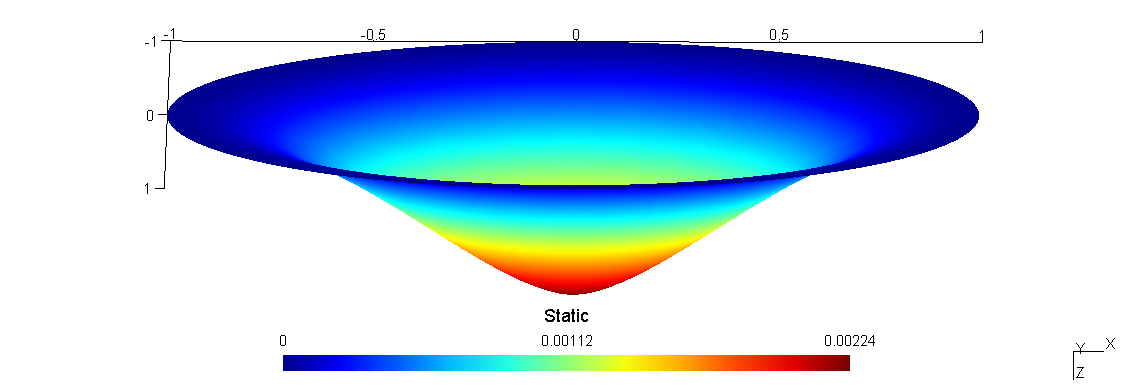
\includegraphics[width=\linewidth,trim={0cm 0 0cm 0},clip]{images/appedix_sim_result/C_BI_P.png}
\caption{Point Load (P)}
\end{subfigure} \vfill
\begin{subfigure}{1\textwidth}
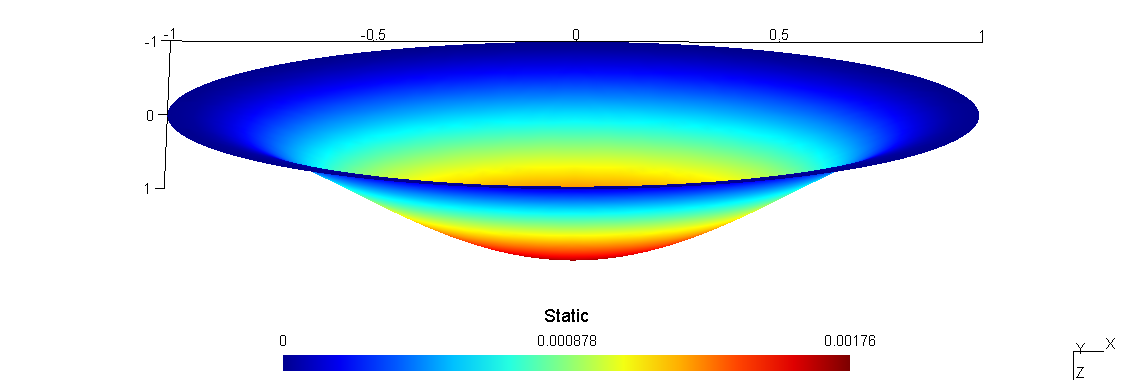
\includegraphics[width=\linewidth,trim={0cm 0 0cm 0},clip]{images/appedix_sim_result/C_BI_q.png}
\caption{Distributed Load (q)}
\end{subfigure}
\caption{Displacement plot of a clamped circular plate}
\end{figure}

\begin{figure}[h!]
\begin{subfigure}{1\textwidth}
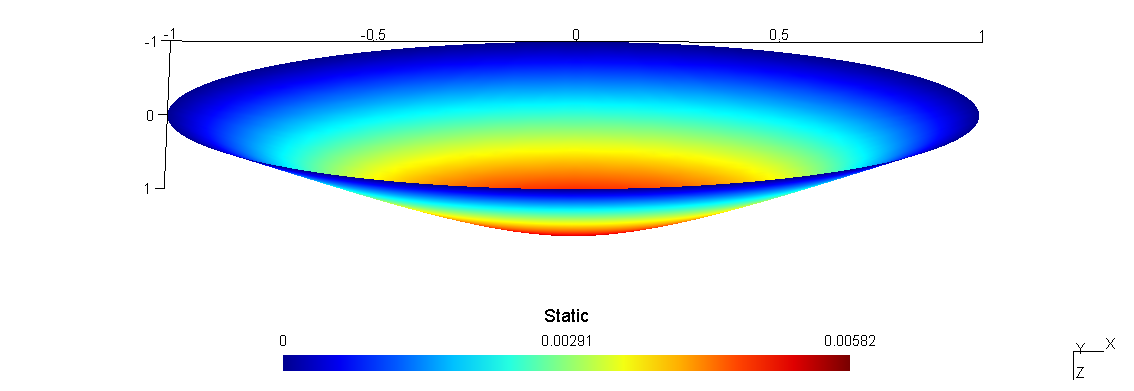
\includegraphics[width=\linewidth,trim={0cm 0 0cm 0},clip]{images/appedix_sim_result/C_SS_P.png}
\caption{Point Load (P)}
\end{subfigure}\vfill
\begin{subfigure}{1\textwidth}
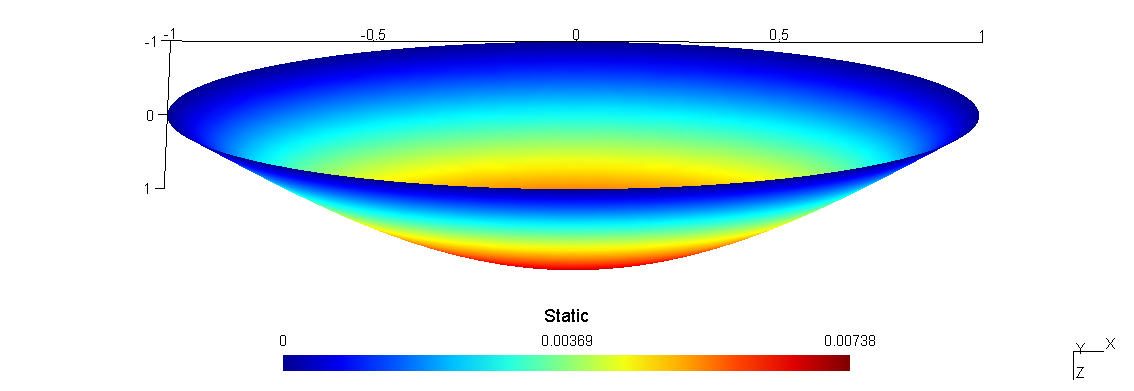
\includegraphics[width=\linewidth,trim={0cm 0 0cm 0},clip]{images/appedix_sim_result/C_SS_q.png}
\caption{Distributed Load (q)}
\end{subfigure}
\caption{Displacement plot of a Simply Supported circular plate}
\end{figure}


\begin{figure}[h!]
\begin{subfigure}{.49\textwidth}
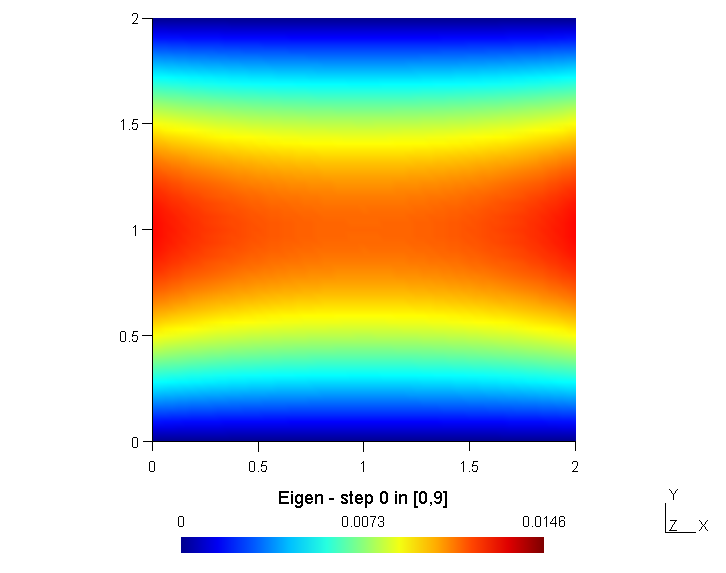
\includegraphics[width=\linewidth,trim={4cm 0 4cm 0},clip]{images/VMP09/1.png}
\caption{Mode Shape 1}
\end{subfigure} \hfill
\begin{subfigure}{.49\textwidth}
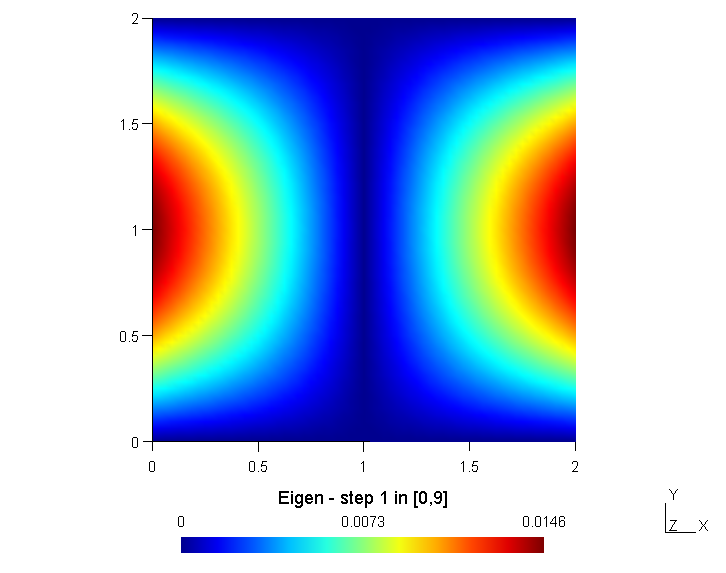
\includegraphics[width=\linewidth,trim={4cm 0 4cm 0},clip]{images/VMP09/2.png}
\caption{Mode Shape 2}
\end{subfigure}\vfill
\begin{subfigure}{.49\textwidth}
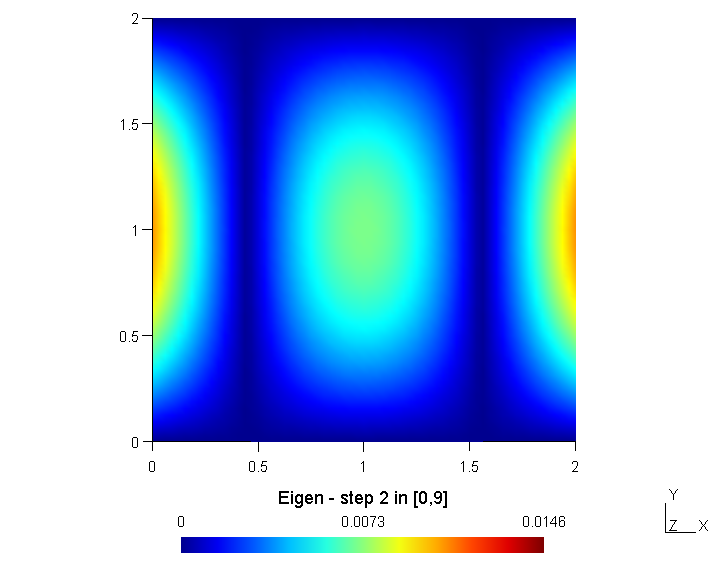
\includegraphics[width=\linewidth,trim={4cm 0 4cm 0},clip]{images/VMP09/3.png}
\caption{Mode Shape 3}
\end{subfigure}\hfill
\begin{subfigure}{.49\textwidth}
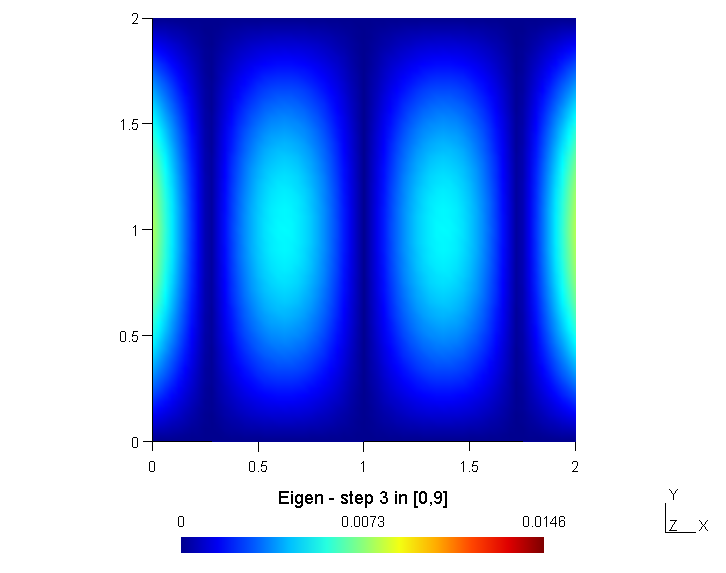
\includegraphics[width=\linewidth,trim={4cm 0 4cm 0},clip]{images/VMP09/4.png}
\caption{Mode Shape 4}
\end{subfigure} 

\caption{Natural Modes of a Square Plate under axial load}
\end{figure}





\begin{figure}[h!]\label{fig:res:FEMvsGAL}
\begin{subfigure}{.98\textwidth}
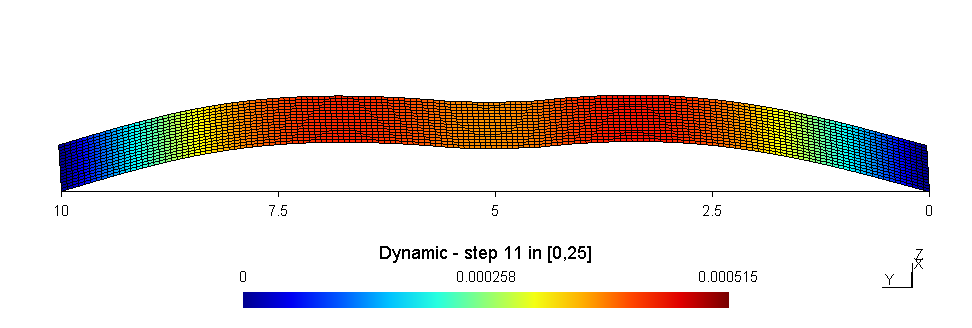
\includegraphics[width=\linewidth,trim={0cm 0 0cm 0},clip]{images/FvsD_F.png}
\caption{Transverse Distributed Load at the middle}
\end{subfigure} \vfill
\begin{subfigure}{.98\textwidth}
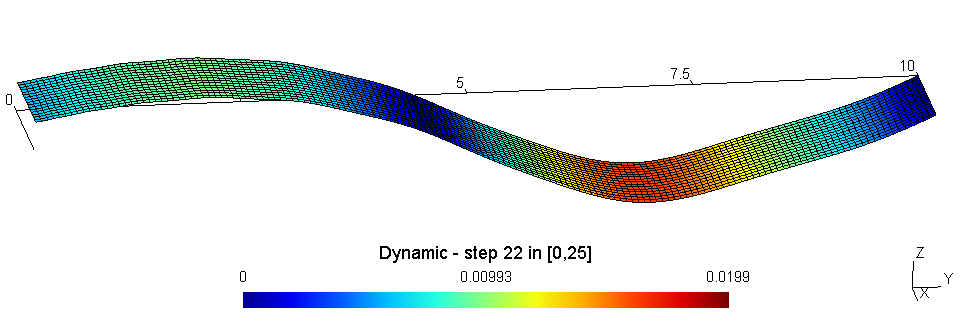
\includegraphics[width=\linewidth,trim={0cm 0 0cm 0},clip]{images/FvsD_D.png}
\caption{Imposed Dirichlet Boundary at $x=0$}
\end{subfigure}

\caption{Displacement plot of a plat under different loads}
\end{figure}





\begin{figure}[h!]

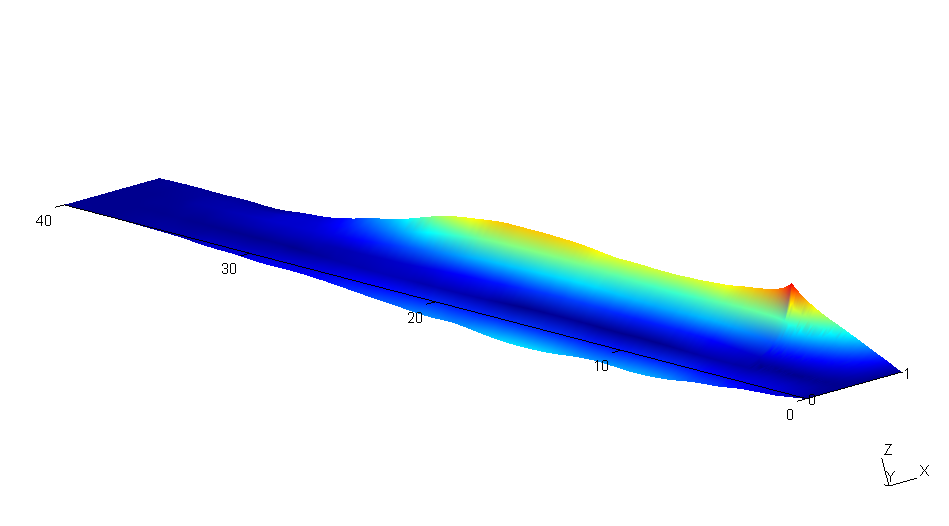
\includegraphics[width=\linewidth,trim={1cm 0 1cm 0},clip]{images/FEMvsGAL.png}



\caption{FE Solution of a metal strip with point load}
\end{figure}



\end{document}